\documentclass[leqno, 12pt]{article}
\usepackage{tikz}
\usepackage{amsmath}
\usepackage{ulem}
\usetikzlibrary{angles,quotes,intersections,arrows.meta,calc}
\usepackage[a4paper, portrait, margin=1cm]{geometry}
\usepackage{multicol}
\usepackage{fancyhdr}

\def \HeadingQuestions {\section*{\Large Name: \underline{\hspace{8cm}} \hfill Date: \underline{\hspace{3cm}}} \vspace{-3mm}
{Parallel lines Angles: Questions} \vspace{1pt}\hrule}

% raise footer with page number; no header
\fancypagestyle{myfancypagestyle}{
  \fancyhf{}% clear all header and footer fields
  \renewcommand{\headrulewidth}{0pt} % no rule under header
  \fancyfoot[C] {\thepage} \setlength{\footskip}{14.5pt} % raise page number 6pt
}
\pagestyle{myfancypagestyle}  % apply myfancypagestyle


\begin{document}
\HeadingQuestions
\begin{multicols}{2}


\begin{equation}
  \text{d} = \text{\dotuline{~~~~~~~}}^\circ

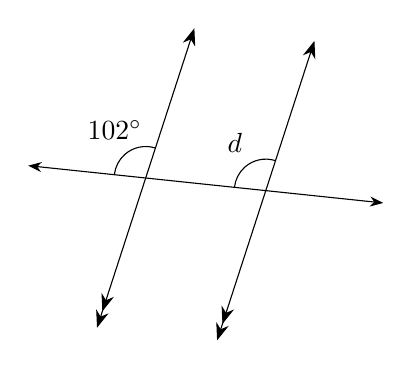
\begin{tikzpicture}[scale=1.0, baseline=(current bounding box.north)]
  \begin{scope}[rotate=174]
    % Draw the first line
    \draw[<->>, >={Stealth[scale=1.3]}, name path=P1] (0, 0) -- (0.8316467632710378, 3.9125904029352223);
    % Draw the second line with the calculated offsets
    \draw[<->>, >={Stealth[scale=1.3]}, name path=P2] (1.533510892297544, 0) -- (2.3651576555685816, 3.9125904029352223);
    % Draw the transversal through the middle of the parallel lines
    \draw[<->, >=Stealth, name path=P3] (-1.0841766183644812, 1.9562952014676112) -- (3.449334273933063, 1.9562952014676112);

    \path [name intersections={of=P1 and P3,by=A}];
    \path [name intersections={of=P2 and P3,by=B}];

    % Draw the angle
    \coordinate (p1s) at (0, 0);
    \coordinate (p1e) at (0.8316467632710378, 3.9125904029352223);
    \coordinate (p2s) at (1.533510892297544, 0);
    \coordinate (p2e) at (2.3651576555685816, 3.9125904029352223);
    \coordinate (ts) at (-1.0841766183644812, 1.9562952014676112);
    \coordinate (te) at (3.449334273933063, 1.9562952014676112);

    % order for vertices go in anticlockwise order te--A--p1e
    \draw pic["$d$", draw=black, -, angle eccentricity=1.8, angle radius=0.4cm] {angle=p1s--A--te};
\draw pic["$102^\circ$", draw=black, -, angle eccentricity=1.8, angle radius=0.4cm] {angle=p2s--B--te};

    % %% Point A
    % \draw pic["$a$", draw=black, -, angle eccentricity=1.5, angle radius=0.4cm] {angle=te--A--p1e};
    % \draw pic["$b$", draw=black, -, angle eccentricity=1.5, angle radius=0.4cm] {angle=p1e--A--ts};
    % \draw pic["$c$", draw=black, -, angle eccentricity=1.5, angle radius=0.4cm] {angle=ts--A--p1s};
    % \draw pic["$d$", draw=black, -, angle eccentricity=1.5, angle radius=0.4cm] {angle=p1s--A--te};

    % %%  Point B
    % \draw pic["$e$", draw=black, -, angle eccentricity=1.5, angle radius=0.4cm] {angle=te--B--p2e};
    % \draw pic["$f$", draw=black, -, angle eccentricity=1.5, angle radius=0.4cm] {angle=p2e--B--ts};
    % \draw pic["$g$", draw=black, -, angle eccentricity=1.5, angle radius=0.4cm] {angle=ts--B--p2s};
    % \draw pic["$h$", draw=black, -, angle eccentricity=1.5, angle radius=0.4cm] {angle=p2s--B--te};

  \end{scope}
\end{tikzpicture}
\vspace{1cm}
\begin{equation}
  \text{f} = \text{\dotuline{~~~~~~~}}^\circ
\end{equation}
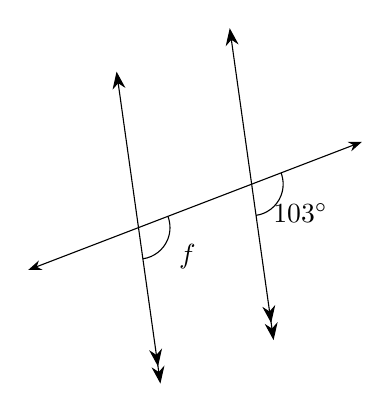
\begin{tikzpicture}[scale=1.0, baseline=(current bounding box.north)]
  \begin{scope}[rotate=201]
    % Draw the first line
    \draw[<->>, >={Stealth[scale=1.3]}, name path=P1] (0, 0) -- (0.8998042173754597, 3.897480259140941);
    % Draw the second line with the calculated offsets
    \draw[<->>, >={Stealth[scale=1.3]}, name path=P2] (1.5394561616900873, 0) -- (2.439260379065547, 3.897480259140941);
    % Draw the transversal through the middle of the parallel lines
    \draw[<->, >=Stealth, name path=P3] (-1.0500978913122703, 1.9487401295704705) -- (3.489358270377817, 1.9487401295704705);

    \path [name intersections={of=P1 and P3,by=A}];
    \path [name intersections={of=P2 and P3,by=B}];

    % Draw the angle
    \coordinate (p1s) at (0, 0);
    \coordinate (p1e) at (0.8998042173754597, 3.897480259140941);
    \coordinate (p2s) at (1.5394561616900873, 0);
    \coordinate (p2e) at (2.439260379065547, 3.897480259140941);
    \coordinate (ts) at (-1.0500978913122703, 1.9487401295704705);
    \coordinate (te) at (3.489358270377817, 1.9487401295704705);

    % order for vertices go in anticlockwise order te--A--p1e
    \draw pic["$f$", draw=black, -, angle eccentricity=1.8, angle radius=0.4cm] {angle=p2e--B--ts};
\draw pic["$103^\circ$", draw=black, -, angle eccentricity=1.8, angle radius=0.4cm] {angle=p1e--A--ts};

    % %% Point A
    % \draw pic["$a$", draw=black, -, angle eccentricity=1.5, angle radius=0.4cm] {angle=te--A--p1e};
    % \draw pic["$b$", draw=black, -, angle eccentricity=1.5, angle radius=0.4cm] {angle=p1e--A--ts};
    % \draw pic["$c$", draw=black, -, angle eccentricity=1.5, angle radius=0.4cm] {angle=ts--A--p1s};
    % \draw pic["$d$", draw=black, -, angle eccentricity=1.5, angle radius=0.4cm] {angle=p1s--A--te};

    % %%  Point B
    % \draw pic["$e$", draw=black, -, angle eccentricity=1.5, angle radius=0.4cm] {angle=te--B--p2e};
    % \draw pic["$f$", draw=black, -, angle eccentricity=1.5, angle radius=0.4cm] {angle=p2e--B--ts};
    % \draw pic["$g$", draw=black, -, angle eccentricity=1.5, angle radius=0.4cm] {angle=ts--B--p2s};
    % \draw pic["$h$", draw=black, -, angle eccentricity=1.5, angle radius=0.4cm] {angle=p2s--B--te};

  \end{scope}
\end{tikzpicture}
\vspace{1cm}
\begin{equation}
  \text{g} = \text{\dotuline{~~~~~~~}}^\circ
\end{equation}
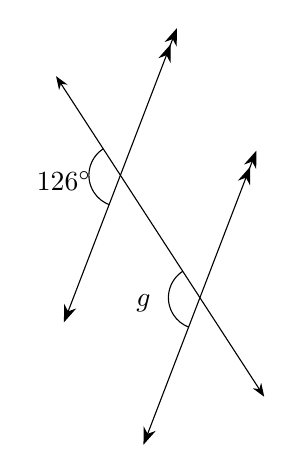
\begin{tikzpicture}[scale=1.0, baseline=(current bounding box.north)]
  \begin{scope}[rotate=303]
    % Draw the first line
    \draw[<->>, >={Stealth[scale=1.3]}, name path=P1] (0, 0) -- (-2.351141009169892, 3.23606797749979);
    % Draw the second line with the calculated offsets
    \draw[<->>, >={Stealth[scale=1.3]}, name path=P2] (1.8541019662496845, 0) -- (-0.4970390429202076, 3.23606797749979);
    % Draw the transversal through the middle of the parallel lines
    \draw[<->, >=Stealth, name path=P3] (-2.6755705045849463, 1.618033988749895) -- (2.1785314616647384, 1.618033988749895);

    \path [name intersections={of=P1 and P3,by=A}];
    \path [name intersections={of=P2 and P3,by=B}];

    % Draw the angle
    \coordinate (p1s) at (0, 0);
    \coordinate (p1e) at (-2.351141009169892, 3.23606797749979);
    \coordinate (p2s) at (1.8541019662496845, 0);
    \coordinate (p2e) at (-0.4970390429202076, 3.23606797749979);
    \coordinate (ts) at (-2.6755705045849463, 1.618033988749895);
    \coordinate (te) at (2.1785314616647384, 1.618033988749895);

    % order for vertices go in anticlockwise order te--A--p1e
    \draw pic["$g$", draw=black, -, angle eccentricity=1.8, angle radius=0.4cm] {angle=ts--B--p2s};
\draw pic["$126^\circ$", draw=black, -, angle eccentricity=1.8, angle radius=0.4cm] {angle=ts--A--p1s};

    % %% Point A
    % \draw pic["$a$", draw=black, -, angle eccentricity=1.5, angle radius=0.4cm] {angle=te--A--p1e};
    % \draw pic["$b$", draw=black, -, angle eccentricity=1.5, angle radius=0.4cm] {angle=p1e--A--ts};
    % \draw pic["$c$", draw=black, -, angle eccentricity=1.5, angle radius=0.4cm] {angle=ts--A--p1s};
    % \draw pic["$d$", draw=black, -, angle eccentricity=1.5, angle radius=0.4cm] {angle=p1s--A--te};

    % %%  Point B
    % \draw pic["$e$", draw=black, -, angle eccentricity=1.5, angle radius=0.4cm] {angle=te--B--p2e};
    % \draw pic["$f$", draw=black, -, angle eccentricity=1.5, angle radius=0.4cm] {angle=p2e--B--ts};
    % \draw pic["$g$", draw=black, -, angle eccentricity=1.5, angle radius=0.4cm] {angle=ts--B--p2s};
    % \draw pic["$h$", draw=black, -, angle eccentricity=1.5, angle radius=0.4cm] {angle=p2s--B--te};

  \end{scope}
\end{tikzpicture}
\vspace{1cm}
\begin{equation}
  \text{a} = \text{\dotuline{~~~~~~~}}^\circ
\end{equation}
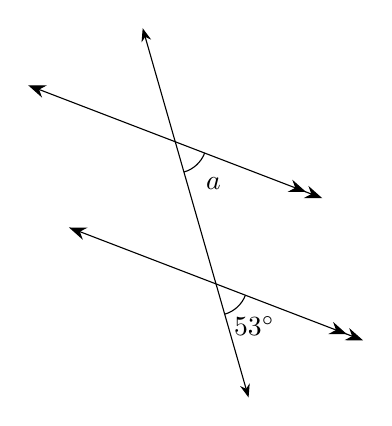
\begin{tikzpicture}[scale=1.0, baseline=(current bounding box.north)]
  \begin{scope}[rotate=286]
    % Draw the first line
    \draw[<->>, >={Stealth[scale=1.3]}, name path=P1] (0, 0) -- (2.4072600926081935, 3.1945420401891713);
    % Draw the second line with the calculated offsets
    \draw[<->>, >={Stealth[scale=1.3]}, name path=P2] (1.8782034872343385, 0) -- (4.285463579842532, 3.1945420401891713);
    % Draw the transversal through the middle of the parallel lines
    \draw[<->, >=Stealth, name path=P3] (-0.296369953695903, 1.5972710200945857) -- (4.581833533538435, 1.5972710200945857);

    \path [name intersections={of=P1 and P3,by=A}];
    \path [name intersections={of=P2 and P3,by=B}];

    % Draw the angle
    \coordinate (p1s) at (0, 0);
    \coordinate (p1e) at (2.4072600926081935, 3.1945420401891713);
    \coordinate (p2s) at (1.8782034872343385, 0);
    \coordinate (p2e) at (4.285463579842532, 3.1945420401891713);
    \coordinate (ts) at (-0.296369953695903, 1.5972710200945857);
    \coordinate (te) at (4.581833533538435, 1.5972710200945857);

    % order for vertices go in anticlockwise order te--A--p1e
    \draw pic["$a$", draw=black, -, angle eccentricity=1.8, angle radius=0.4cm] {angle=te--A--p1e};
\draw pic["$53^\circ$", draw=black, -, angle eccentricity=1.8, angle radius=0.4cm] {angle=te--B--p2e};

    % %% Point A
    % \draw pic["$a$", draw=black, -, angle eccentricity=1.5, angle radius=0.4cm] {angle=te--A--p1e};
    % \draw pic["$b$", draw=black, -, angle eccentricity=1.5, angle radius=0.4cm] {angle=p1e--A--ts};
    % \draw pic["$c$", draw=black, -, angle eccentricity=1.5, angle radius=0.4cm] {angle=ts--A--p1s};
    % \draw pic["$d$", draw=black, -, angle eccentricity=1.5, angle radius=0.4cm] {angle=p1s--A--te};

    % %%  Point B
    % \draw pic["$e$", draw=black, -, angle eccentricity=1.5, angle radius=0.4cm] {angle=te--B--p2e};
    % \draw pic["$f$", draw=black, -, angle eccentricity=1.5, angle radius=0.4cm] {angle=p2e--B--ts};
    % \draw pic["$g$", draw=black, -, angle eccentricity=1.5, angle radius=0.4cm] {angle=ts--B--p2s};
    % \draw pic["$h$", draw=black, -, angle eccentricity=1.5, angle radius=0.4cm] {angle=p2s--B--te};

  \end{scope}
\end{tikzpicture}
\vspace{1cm}
\begin{equation}
  \text{e} = \text{\dotuline{~~~~~~~}}^\circ
\end{equation}
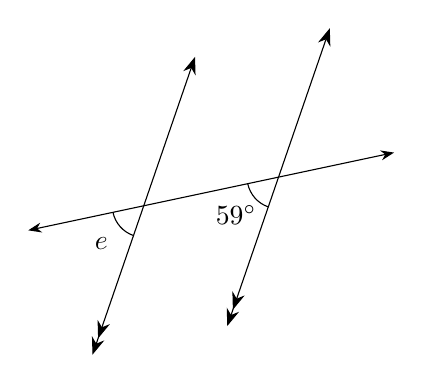
\begin{tikzpicture}[scale=1.0, baseline=(current bounding box.north)]
  \begin{scope}[rotate=192]
    % Draw the first line
    \draw[<->>, >={Stealth[scale=1.3]}, name path=P1] (0, 0) -- (2.0601522996402166, 3.4286692028084493);
    % Draw the second line with the calculated offsets
    \draw[<->>, >={Stealth[scale=1.3]}, name path=P2] (1.7499500958229957, 0) -- (3.810102395463212, 3.4286692028084493);
    % Draw the transversal through the middle of the parallel lines
    \draw[<->, >=Stealth, name path=P3] (-0.4699238501798919, 1.7143346014042247) -- (4.2800262456431035, 1.7143346014042247);

    \path [name intersections={of=P1 and P3,by=A}];
    \path [name intersections={of=P2 and P3,by=B}];

    % Draw the angle
    \coordinate (p1s) at (0, 0);
    \coordinate (p1e) at (2.0601522996402166, 3.4286692028084493);
    \coordinate (p2s) at (1.7499500958229957, 0);
    \coordinate (p2e) at (3.810102395463212, 3.4286692028084493);
    \coordinate (ts) at (-0.4699238501798919, 1.7143346014042247);
    \coordinate (te) at (4.2800262456431035, 1.7143346014042247);

    % order for vertices go in anticlockwise order te--A--p1e
    \draw pic["$e$", draw=black, -, angle eccentricity=1.8, angle radius=0.4cm] {angle=te--B--p2e};
\draw pic["$59^\circ$", draw=black, -, angle eccentricity=1.8, angle radius=0.4cm] {angle=te--A--p1e};

    % %% Point A
    % \draw pic["$a$", draw=black, -, angle eccentricity=1.5, angle radius=0.4cm] {angle=te--A--p1e};
    % \draw pic["$b$", draw=black, -, angle eccentricity=1.5, angle radius=0.4cm] {angle=p1e--A--ts};
    % \draw pic["$c$", draw=black, -, angle eccentricity=1.5, angle radius=0.4cm] {angle=ts--A--p1s};
    % \draw pic["$d$", draw=black, -, angle eccentricity=1.5, angle radius=0.4cm] {angle=p1s--A--te};

    % %%  Point B
    % \draw pic["$e$", draw=black, -, angle eccentricity=1.5, angle radius=0.4cm] {angle=te--B--p2e};
    % \draw pic["$f$", draw=black, -, angle eccentricity=1.5, angle radius=0.4cm] {angle=p2e--B--ts};
    % \draw pic["$g$", draw=black, -, angle eccentricity=1.5, angle radius=0.4cm] {angle=ts--B--p2s};
    % \draw pic["$h$", draw=black, -, angle eccentricity=1.5, angle radius=0.4cm] {angle=p2s--B--te};

  \end{scope}
\end{tikzpicture}
\vspace{1cm}
\begin{equation}
  \text{f} = \text{\dotuline{~~~~~~~}}^\circ
\end{equation}
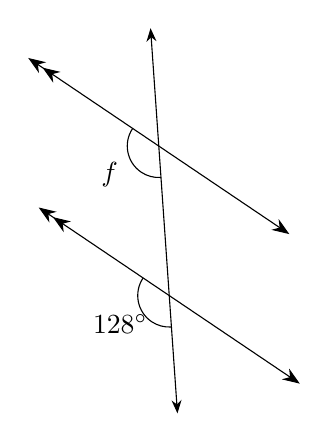
\begin{tikzpicture}[scale=1.0, baseline=(current bounding box.north)]
  \begin{scope}[rotate=94]
    % Draw the first line
    \draw[<->>, >={Stealth[scale=1.3]}, name path=P1] (0, 0) -- (2.462645901302633, 3.152043014426888);
    % Draw the second line with the calculated offsets
    \draw[<->>, >={Stealth[scale=1.3]}, name path=P2] (1.903527322608868, 0) -- (4.366173223911501, 3.152043014426888);
    % Draw the transversal through the middle of the parallel lines
    \draw[<->, >=Stealth, name path=P3] (-0.26867704934868364, 1.576021507213444) -- (4.634850273260184, 1.576021507213444);

    \path [name intersections={of=P1 and P3,by=A}];
    \path [name intersections={of=P2 and P3,by=B}];

    % Draw the angle
    \coordinate (p1s) at (0, 0);
    \coordinate (p1e) at (2.462645901302633, 3.152043014426888);
    \coordinate (p2s) at (1.903527322608868, 0);
    \coordinate (p2e) at (4.366173223911501, 3.152043014426888);
    \coordinate (ts) at (-0.26867704934868364, 1.576021507213444);
    \coordinate (te) at (4.634850273260184, 1.576021507213444);

    % order for vertices go in anticlockwise order te--A--p1e
    \draw pic["$f$", draw=black, -, angle eccentricity=1.8, angle radius=0.4cm] {angle=p2e--B--ts};
\draw pic["$128^\circ$", draw=black, -, angle eccentricity=1.8, angle radius=0.4cm] {angle=p1e--A--ts};

    % %% Point A
    % \draw pic["$a$", draw=black, -, angle eccentricity=1.5, angle radius=0.4cm] {angle=te--A--p1e};
    % \draw pic["$b$", draw=black, -, angle eccentricity=1.5, angle radius=0.4cm] {angle=p1e--A--ts};
    % \draw pic["$c$", draw=black, -, angle eccentricity=1.5, angle radius=0.4cm] {angle=ts--A--p1s};
    % \draw pic["$d$", draw=black, -, angle eccentricity=1.5, angle radius=0.4cm] {angle=p1s--A--te};

    % %%  Point B
    % \draw pic["$e$", draw=black, -, angle eccentricity=1.5, angle radius=0.4cm] {angle=te--B--p2e};
    % \draw pic["$f$", draw=black, -, angle eccentricity=1.5, angle radius=0.4cm] {angle=p2e--B--ts};
    % \draw pic["$g$", draw=black, -, angle eccentricity=1.5, angle radius=0.4cm] {angle=ts--B--p2s};
    % \draw pic["$h$", draw=black, -, angle eccentricity=1.5, angle radius=0.4cm] {angle=p2s--B--te};

  \end{scope}
\end{tikzpicture}
\vspace{1cm}
\begin{equation}
  \text{h} = \text{\dotuline{~~~~~~~}}^\circ
\end{equation}
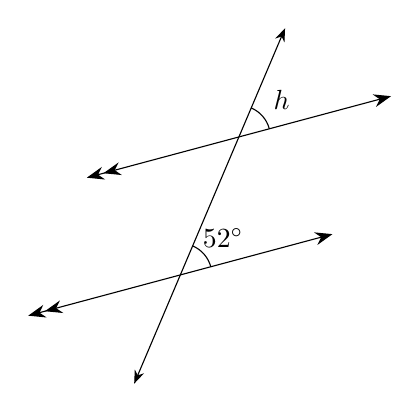
\begin{tikzpicture}[scale=1.0, baseline=(current bounding box.north)]
  \begin{scope}[rotate=67]
    % Draw the first line
    \draw[<->>, >={Stealth[scale=1.3]}, name path=P1] (0, 0) -- (-2.462645901302633, 3.152043014426888);
    % Draw the second line with the calculated offsets
    \draw[<->>, >={Stealth[scale=1.3]}, name path=P2] (1.903527322608868, 0) -- (-0.5591185786937651, 3.152043014426888);
    % Draw the transversal through the middle of the parallel lines
    \draw[<->, >=Stealth, name path=P3] (-2.7313229506513164, 1.576021507213444) -- (2.1722043719575517, 1.576021507213444);

    \path [name intersections={of=P1 and P3,by=A}];
    \path [name intersections={of=P2 and P3,by=B}];

    % Draw the angle
    \coordinate (p1s) at (0, 0);
    \coordinate (p1e) at (-2.462645901302633, 3.152043014426888);
    \coordinate (p2s) at (1.903527322608868, 0);
    \coordinate (p2e) at (-0.5591185786937651, 3.152043014426888);
    \coordinate (ts) at (-2.7313229506513164, 1.576021507213444);
    \coordinate (te) at (2.1722043719575517, 1.576021507213444);

    % order for vertices go in anticlockwise order te--A--p1e
    \draw pic["$h$", draw=black, -, angle eccentricity=1.8, angle radius=0.4cm] {angle=p2s--B--te};
\draw pic["$52^\circ$", draw=black, -, angle eccentricity=1.8, angle radius=0.4cm] {angle=p1s--A--te};

    % %% Point A
    % \draw pic["$a$", draw=black, -, angle eccentricity=1.5, angle radius=0.4cm] {angle=te--A--p1e};
    % \draw pic["$b$", draw=black, -, angle eccentricity=1.5, angle radius=0.4cm] {angle=p1e--A--ts};
    % \draw pic["$c$", draw=black, -, angle eccentricity=1.5, angle radius=0.4cm] {angle=ts--A--p1s};
    % \draw pic["$d$", draw=black, -, angle eccentricity=1.5, angle radius=0.4cm] {angle=p1s--A--te};

    % %%  Point B
    % \draw pic["$e$", draw=black, -, angle eccentricity=1.5, angle radius=0.4cm] {angle=te--B--p2e};
    % \draw pic["$f$", draw=black, -, angle eccentricity=1.5, angle radius=0.4cm] {angle=p2e--B--ts};
    % \draw pic["$g$", draw=black, -, angle eccentricity=1.5, angle radius=0.4cm] {angle=ts--B--p2s};
    % \draw pic["$h$", draw=black, -, angle eccentricity=1.5, angle radius=0.4cm] {angle=p2s--B--te};

  \end{scope}
\end{tikzpicture}
\vspace{1cm}
\begin{equation}
  \text{d} = \text{\dotuline{~~~~~~~}}^\circ
\end{equation}
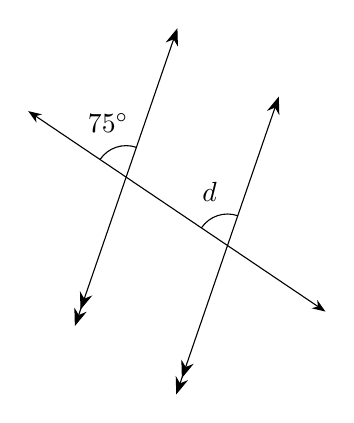
\begin{tikzpicture}[scale=1.0, baseline=(current bounding box.north)]
  \begin{scope}[rotate=146]
    % Draw the first line
    \draw[<->>, >={Stealth[scale=1.3]}, name path=P1] (0, 0) -- (-1.0352761804100834, 3.8637033051562732);
    % Draw the second line with the calculated offsets
    \draw[<->>, >={Stealth[scale=1.3]}, name path=P2] (1.5529142706151244, 0) -- (0.517638090205041, 3.8637033051562732);
    % Draw the transversal through the middle of the parallel lines
    \draw[<->, >=Stealth, name path=P3] (-2.0176380902050415, 1.9318516525781366) -- (2.535276180410083, 1.9318516525781366);

    \path [name intersections={of=P1 and P3,by=A}];
    \path [name intersections={of=P2 and P3,by=B}];

    % Draw the angle
    \coordinate (p1s) at (0, 0);
    \coordinate (p1e) at (-1.0352761804100834, 3.8637033051562732);
    \coordinate (p2s) at (1.5529142706151244, 0);
    \coordinate (p2e) at (0.517638090205041, 3.8637033051562732);
    \coordinate (ts) at (-2.0176380902050415, 1.9318516525781366);
    \coordinate (te) at (2.535276180410083, 1.9318516525781366);

    % order for vertices go in anticlockwise order te--A--p1e
    \draw pic["$d$", draw=black, -, angle eccentricity=1.8, angle radius=0.4cm] {angle=p1s--A--te};
\draw pic["$75^\circ$", draw=black, -, angle eccentricity=1.8, angle radius=0.4cm] {angle=p2s--B--te};

    % %% Point A
    % \draw pic["$a$", draw=black, -, angle eccentricity=1.5, angle radius=0.4cm] {angle=te--A--p1e};
    % \draw pic["$b$", draw=black, -, angle eccentricity=1.5, angle radius=0.4cm] {angle=p1e--A--ts};
    % \draw pic["$c$", draw=black, -, angle eccentricity=1.5, angle radius=0.4cm] {angle=ts--A--p1s};
    % \draw pic["$d$", draw=black, -, angle eccentricity=1.5, angle radius=0.4cm] {angle=p1s--A--te};

    % %%  Point B
    % \draw pic["$e$", draw=black, -, angle eccentricity=1.5, angle radius=0.4cm] {angle=te--B--p2e};
    % \draw pic["$f$", draw=black, -, angle eccentricity=1.5, angle radius=0.4cm] {angle=p2e--B--ts};
    % \draw pic["$g$", draw=black, -, angle eccentricity=1.5, angle radius=0.4cm] {angle=ts--B--p2s};
    % \draw pic["$h$", draw=black, -, angle eccentricity=1.5, angle radius=0.4cm] {angle=p2s--B--te};

  \end{scope}
\end{tikzpicture}
\vspace{1cm}
\begin{equation}
  \text{g} = \text{\dotuline{~~~~~~~}}^\circ
\end{equation}
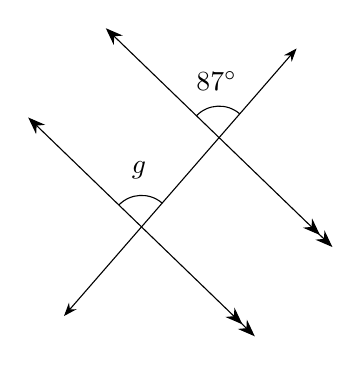
\begin{tikzpicture}[scale=1.0, baseline=(current bounding box.north)]
  \begin{scope}[rotate=229]
    % Draw the first line
    \draw[<->>, >={Stealth[scale=1.3]}, name path=P1] (0, 0) -- (0.20934382497177587, 3.9945181390182953);
    % Draw the second line with the calculated offsets
    \draw[<->>, >={Stealth[scale=1.3]}, name path=P2] (1.5020585189968816, 0) -- (1.7114023439686574, 3.9945181390182953);
    % Draw the transversal through the middle of the parallel lines
    \draw[<->, >=Stealth, name path=P3] (-1.395328087514112, 1.9972590695091477) -- (3.1067304314827697, 1.9972590695091477);

    \path [name intersections={of=P1 and P3,by=A}];
    \path [name intersections={of=P2 and P3,by=B}];

    % Draw the angle
    \coordinate (p1s) at (0, 0);
    \coordinate (p1e) at (0.20934382497177587, 3.9945181390182953);
    \coordinate (p2s) at (1.5020585189968816, 0);
    \coordinate (p2e) at (1.7114023439686574, 3.9945181390182953);
    \coordinate (ts) at (-1.395328087514112, 1.9972590695091477);
    \coordinate (te) at (3.1067304314827697, 1.9972590695091477);

    % order for vertices go in anticlockwise order te--A--p1e
    \draw pic["$g$", draw=black, -, angle eccentricity=1.8, angle radius=0.4cm] {angle=ts--B--p2s};
\draw pic["$87^\circ$", draw=black, -, angle eccentricity=1.8, angle radius=0.4cm] {angle=ts--A--p1s};

    % %% Point A
    % \draw pic["$a$", draw=black, -, angle eccentricity=1.5, angle radius=0.4cm] {angle=te--A--p1e};
    % \draw pic["$b$", draw=black, -, angle eccentricity=1.5, angle radius=0.4cm] {angle=p1e--A--ts};
    % \draw pic["$c$", draw=black, -, angle eccentricity=1.5, angle radius=0.4cm] {angle=ts--A--p1s};
    % \draw pic["$d$", draw=black, -, angle eccentricity=1.5, angle radius=0.4cm] {angle=p1s--A--te};

    % %%  Point B
    % \draw pic["$e$", draw=black, -, angle eccentricity=1.5, angle radius=0.4cm] {angle=te--B--p2e};
    % \draw pic["$f$", draw=black, -, angle eccentricity=1.5, angle radius=0.4cm] {angle=p2e--B--ts};
    % \draw pic["$g$", draw=black, -, angle eccentricity=1.5, angle radius=0.4cm] {angle=ts--B--p2s};
    % \draw pic["$h$", draw=black, -, angle eccentricity=1.5, angle radius=0.4cm] {angle=p2s--B--te};

  \end{scope}
\end{tikzpicture}
\vspace{1cm}
\begin{equation}
  \text{e} = \text{\dotuline{~~~~~~~}}^\circ
\end{equation}
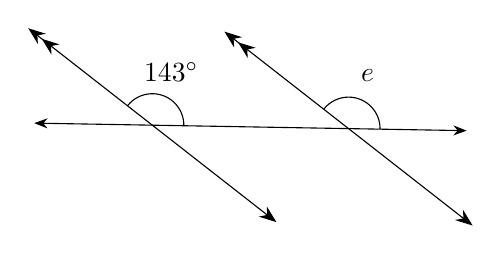
\begin{tikzpicture}[scale=1.0, baseline=(current bounding box.north)]
  \begin{scope}[rotate=359]
    % Draw the first line
    \draw[<->>, >={Stealth[scale=1.3]}, name path=P1] (0, 0) -- (-3.1945420401891718, 2.4072600926081926);
    % Draw the second line with the calculated offsets
    \draw[<->>, >={Stealth[scale=1.3]}, name path=P2] (2.492460211683725, 0) -- (-0.7020818285054466, 2.4072600926081926);
    % Draw the transversal through the middle of the parallel lines
    \draw[<->, >=Stealth, name path=P3] (-3.0972710200945857, 1.2036300463040963) -- (2.3951891915891386, 1.2036300463040963);

    \path [name intersections={of=P1 and P3,by=A}];
    \path [name intersections={of=P2 and P3,by=B}];

    % Draw the angle
    \coordinate (p1s) at (0, 0);
    \coordinate (p1e) at (-3.1945420401891718, 2.4072600926081926);
    \coordinate (p2s) at (2.492460211683725, 0);
    \coordinate (p2e) at (-0.7020818285054466, 2.4072600926081926);
    \coordinate (ts) at (-3.0972710200945857, 1.2036300463040963);
    \coordinate (te) at (2.3951891915891386, 1.2036300463040963);

    % order for vertices go in anticlockwise order te--A--p1e
    \draw pic["$e$", draw=black, -, angle eccentricity=1.8, angle radius=0.4cm] {angle=te--B--p2e};
\draw pic["$143^\circ$", draw=black, -, angle eccentricity=1.8, angle radius=0.4cm] {angle=te--A--p1e};

    % %% Point A
    % \draw pic["$a$", draw=black, -, angle eccentricity=1.5, angle radius=0.4cm] {angle=te--A--p1e};
    % \draw pic["$b$", draw=black, -, angle eccentricity=1.5, angle radius=0.4cm] {angle=p1e--A--ts};
    % \draw pic["$c$", draw=black, -, angle eccentricity=1.5, angle radius=0.4cm] {angle=ts--A--p1s};
    % \draw pic["$d$", draw=black, -, angle eccentricity=1.5, angle radius=0.4cm] {angle=p1s--A--te};

    % %%  Point B
    % \draw pic["$e$", draw=black, -, angle eccentricity=1.5, angle radius=0.4cm] {angle=te--B--p2e};
    % \draw pic["$f$", draw=black, -, angle eccentricity=1.5, angle radius=0.4cm] {angle=p2e--B--ts};
    % \draw pic["$g$", draw=black, -, angle eccentricity=1.5, angle radius=0.4cm] {angle=ts--B--p2s};
    % \draw pic["$h$", draw=black, -, angle eccentricity=1.5, angle radius=0.4cm] {angle=p2s--B--te};

  \end{scope}
\end{tikzpicture}
\vspace{1cm}
\begin{equation}
  \text{e} = \text{\dotuline{~~~~~~~}}^\circ
\end{equation}
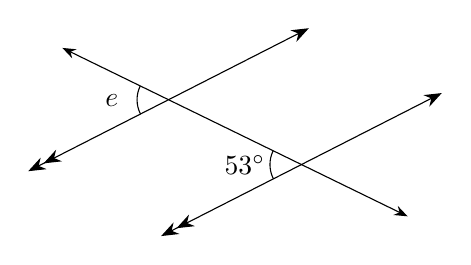
\begin{tikzpicture}[scale=1.0, baseline=(current bounding box.north)]
  \begin{scope}[rotate=154]
    % Draw the first line
    \draw[<->>, >={Stealth[scale=1.3]}, name path=P1] (0, 0) -- (2.4072600926081935, 3.1945420401891713);
    % Draw the second line with the calculated offsets
    \draw[<->>, >={Stealth[scale=1.3]}, name path=P2] (1.8782034872343385, 0) -- (4.285463579842532, 3.1945420401891713);
    % Draw the transversal through the middle of the parallel lines
    \draw[<->, >=Stealth, name path=P3] (-0.296369953695903, 1.5972710200945857) -- (4.581833533538435, 1.5972710200945857);

    \path [name intersections={of=P1 and P3,by=A}];
    \path [name intersections={of=P2 and P3,by=B}];

    % Draw the angle
    \coordinate (p1s) at (0, 0);
    \coordinate (p1e) at (2.4072600926081935, 3.1945420401891713);
    \coordinate (p2s) at (1.8782034872343385, 0);
    \coordinate (p2e) at (4.285463579842532, 3.1945420401891713);
    \coordinate (ts) at (-0.296369953695903, 1.5972710200945857);
    \coordinate (te) at (4.581833533538435, 1.5972710200945857);

    % order for vertices go in anticlockwise order te--A--p1e
    \draw pic["$e$", draw=black, -, angle eccentricity=1.8, angle radius=0.4cm] {angle=te--B--p2e};
\draw pic["$53^\circ$", draw=black, -, angle eccentricity=1.8, angle radius=0.4cm] {angle=te--A--p1e};

    % %% Point A
    % \draw pic["$a$", draw=black, -, angle eccentricity=1.5, angle radius=0.4cm] {angle=te--A--p1e};
    % \draw pic["$b$", draw=black, -, angle eccentricity=1.5, angle radius=0.4cm] {angle=p1e--A--ts};
    % \draw pic["$c$", draw=black, -, angle eccentricity=1.5, angle radius=0.4cm] {angle=ts--A--p1s};
    % \draw pic["$d$", draw=black, -, angle eccentricity=1.5, angle radius=0.4cm] {angle=p1s--A--te};

    % %%  Point B
    % \draw pic["$e$", draw=black, -, angle eccentricity=1.5, angle radius=0.4cm] {angle=te--B--p2e};
    % \draw pic["$f$", draw=black, -, angle eccentricity=1.5, angle radius=0.4cm] {angle=p2e--B--ts};
    % \draw pic["$g$", draw=black, -, angle eccentricity=1.5, angle radius=0.4cm] {angle=ts--B--p2s};
    % \draw pic["$h$", draw=black, -, angle eccentricity=1.5, angle radius=0.4cm] {angle=p2s--B--te};

  \end{scope}
\end{tikzpicture}
\vspace{1cm}
\begin{equation}
  \text{b} = \text{\dotuline{~~~~~~~}}^\circ
\end{equation}
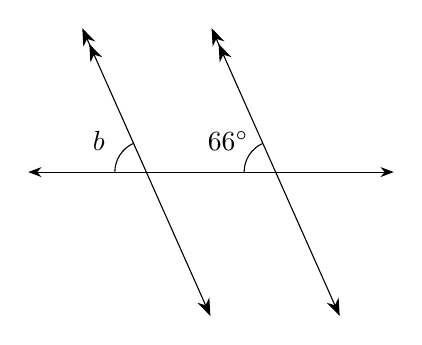
\begin{tikzpicture}[scale=1.0, baseline=(current bounding box.north)]
  \begin{scope}[rotate=0]
    % Draw the first line
    \draw[<->>, >={Stealth[scale=1.3]}, name path=P1] (0, 0) -- (-1.626946572303201, 3.6541818305704035);
    % Draw the second line with the calculated offsets
    \draw[<->>, >={Stealth[scale=1.3]}, name path=P2] (1.6419544177590701, 0) -- (0.015007845455869084, 3.6541818305704035);
    % Draw the transversal through the middle of the parallel lines
    \draw[<->, >=Stealth, name path=P3] (-2.3134732861516003, 1.8270909152852017) -- (2.32848113160747, 1.8270909152852017);

    \path [name intersections={of=P1 and P3,by=A}];
    \path [name intersections={of=P2 and P3,by=B}];

    % Draw the angle
    \coordinate (p1s) at (0, 0);
    \coordinate (p1e) at (-1.626946572303201, 3.6541818305704035);
    \coordinate (p2s) at (1.6419544177590701, 0);
    \coordinate (p2e) at (0.015007845455869084, 3.6541818305704035);
    \coordinate (ts) at (-2.3134732861516003, 1.8270909152852017);
    \coordinate (te) at (2.32848113160747, 1.8270909152852017);

    % order for vertices go in anticlockwise order te--A--p1e
    \draw pic["$b$", draw=black, -, angle eccentricity=1.8, angle radius=0.4cm] {angle=p1e--A--ts};
\draw pic["$66^\circ$", draw=black, -, angle eccentricity=1.8, angle radius=0.4cm] {angle=p2e--B--ts};

    % %% Point A
    % \draw pic["$a$", draw=black, -, angle eccentricity=1.5, angle radius=0.4cm] {angle=te--A--p1e};
    % \draw pic["$b$", draw=black, -, angle eccentricity=1.5, angle radius=0.4cm] {angle=p1e--A--ts};
    % \draw pic["$c$", draw=black, -, angle eccentricity=1.5, angle radius=0.4cm] {angle=ts--A--p1s};
    % \draw pic["$d$", draw=black, -, angle eccentricity=1.5, angle radius=0.4cm] {angle=p1s--A--te};

    % %%  Point B
    % \draw pic["$e$", draw=black, -, angle eccentricity=1.5, angle radius=0.4cm] {angle=te--B--p2e};
    % \draw pic["$f$", draw=black, -, angle eccentricity=1.5, angle radius=0.4cm] {angle=p2e--B--ts};
    % \draw pic["$g$", draw=black, -, angle eccentricity=1.5, angle radius=0.4cm] {angle=ts--B--p2s};
    % \draw pic["$h$", draw=black, -, angle eccentricity=1.5, angle radius=0.4cm] {angle=p2s--B--te};

  \end{scope}
\end{tikzpicture}
\vspace{1cm}

\end{multicols}
\end{document}
